\vspace{-1cm}
\chapter{Superexchange mechanism and quantum manybody excitations in the archetypal di-Cu oxo-bridge}
\label{Hemocyanin}
\vspace{-1cm}

In this work, we study the electronic structure of the hemocyanin protein, where in particular we study the 59-atom protein core using density functional theory + dynamical mean field theory (DFT+DMFT). Here, we find that the hemocyanin protein utilises electronic correlation effects in performing its function of oxygen transport. By treating the copper 3\textit{d} electrons in the hemocyanin functional site using DMFT, we recover experimentally observed singlet electronic ground state. This work allows the transferability of the DFT+DMFT approach to the quantum treatment of the entire protein, using linear-scaling DFT. The importance of accurate simulation of the Hemocyanin core is in understanding how biological systems have evolved to function through quantum biology, as well as its use in biomimetic applications in engineering.\cite{al2020superexchange} \edit{Contributions for this work are as follows: \textbf{Cedric Weber} and \textbf{Mohamed Ali al-Badri} conceived and planned the research. \textbf{Mohamed Ali al-Badri, Edward Linscott} and \textbf{Cedric Weber} performed the calculations. \textbf{Mohamed Ali al-Badri
Edward Linscott, Antoine Georges, Daniel J. Cole} and \textbf{Cedric Weber} analysed the data and contributed to the final manuscript. \textbf{Edward Linscott} independently ran the NBO analysis (Supp. Fig.~3) and the scaling calculations (Supp. Fig.~5).}

%Contributions for this work are as follows: \textbf{Cedric Weber and Mohamed Ali al-Badri} conceived and planned the research. \textbf{Mohamed Ali al-Badri, Edward Linscott} and \textbf{Cedric Weber} performed the calculations. \textbf{Mohamed Ali al-Badri, Edward Linscott, Antoine Georges, Daniel J. Cole} and \textbf{Cedric Weber} analysed the data and contributed to the final manuscript. \edit{Edward Linscott independently ran the Natural Bonding Orbital (NBO) analysis (Supplementary Fig.~3) and the scaling calculations (Supplementary Fig.~5).}
%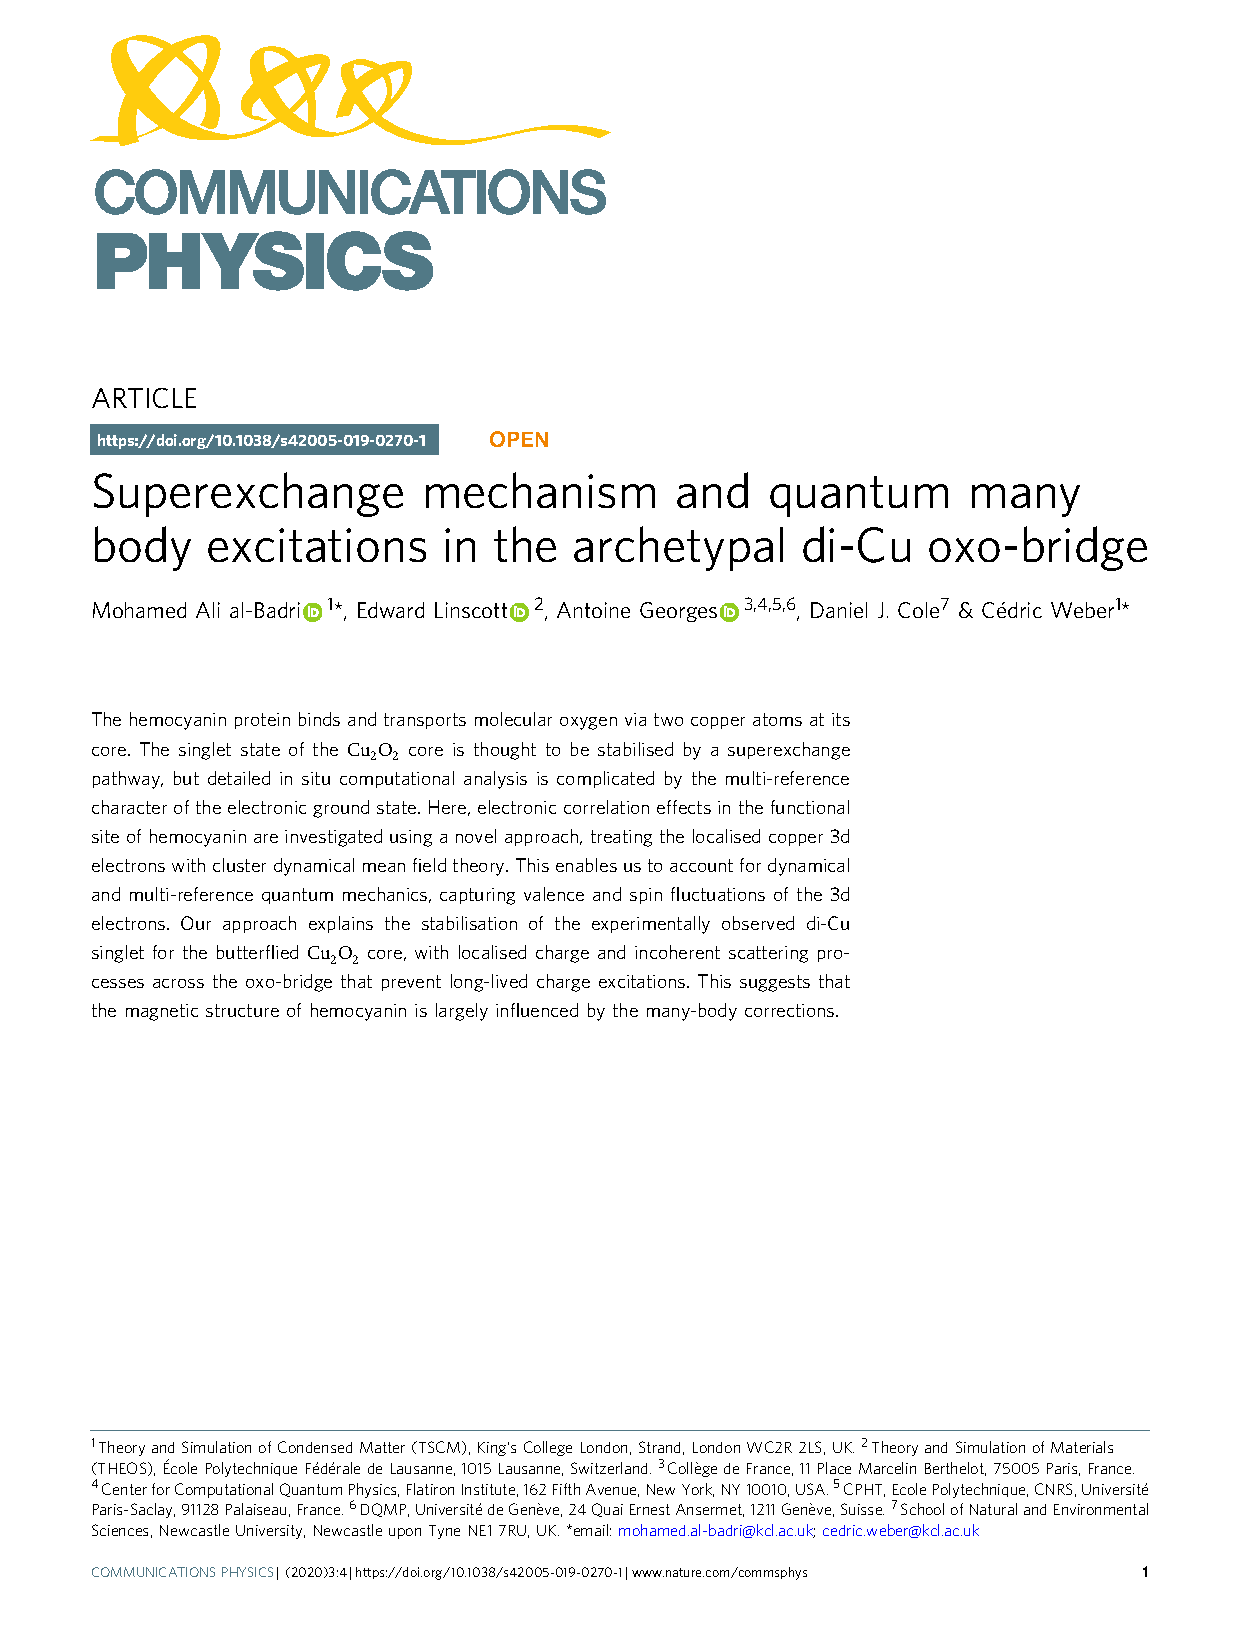
\includepdf[pages=-, offset=75 -75]{PDF_PAPERS/hemocyanin.pdf}


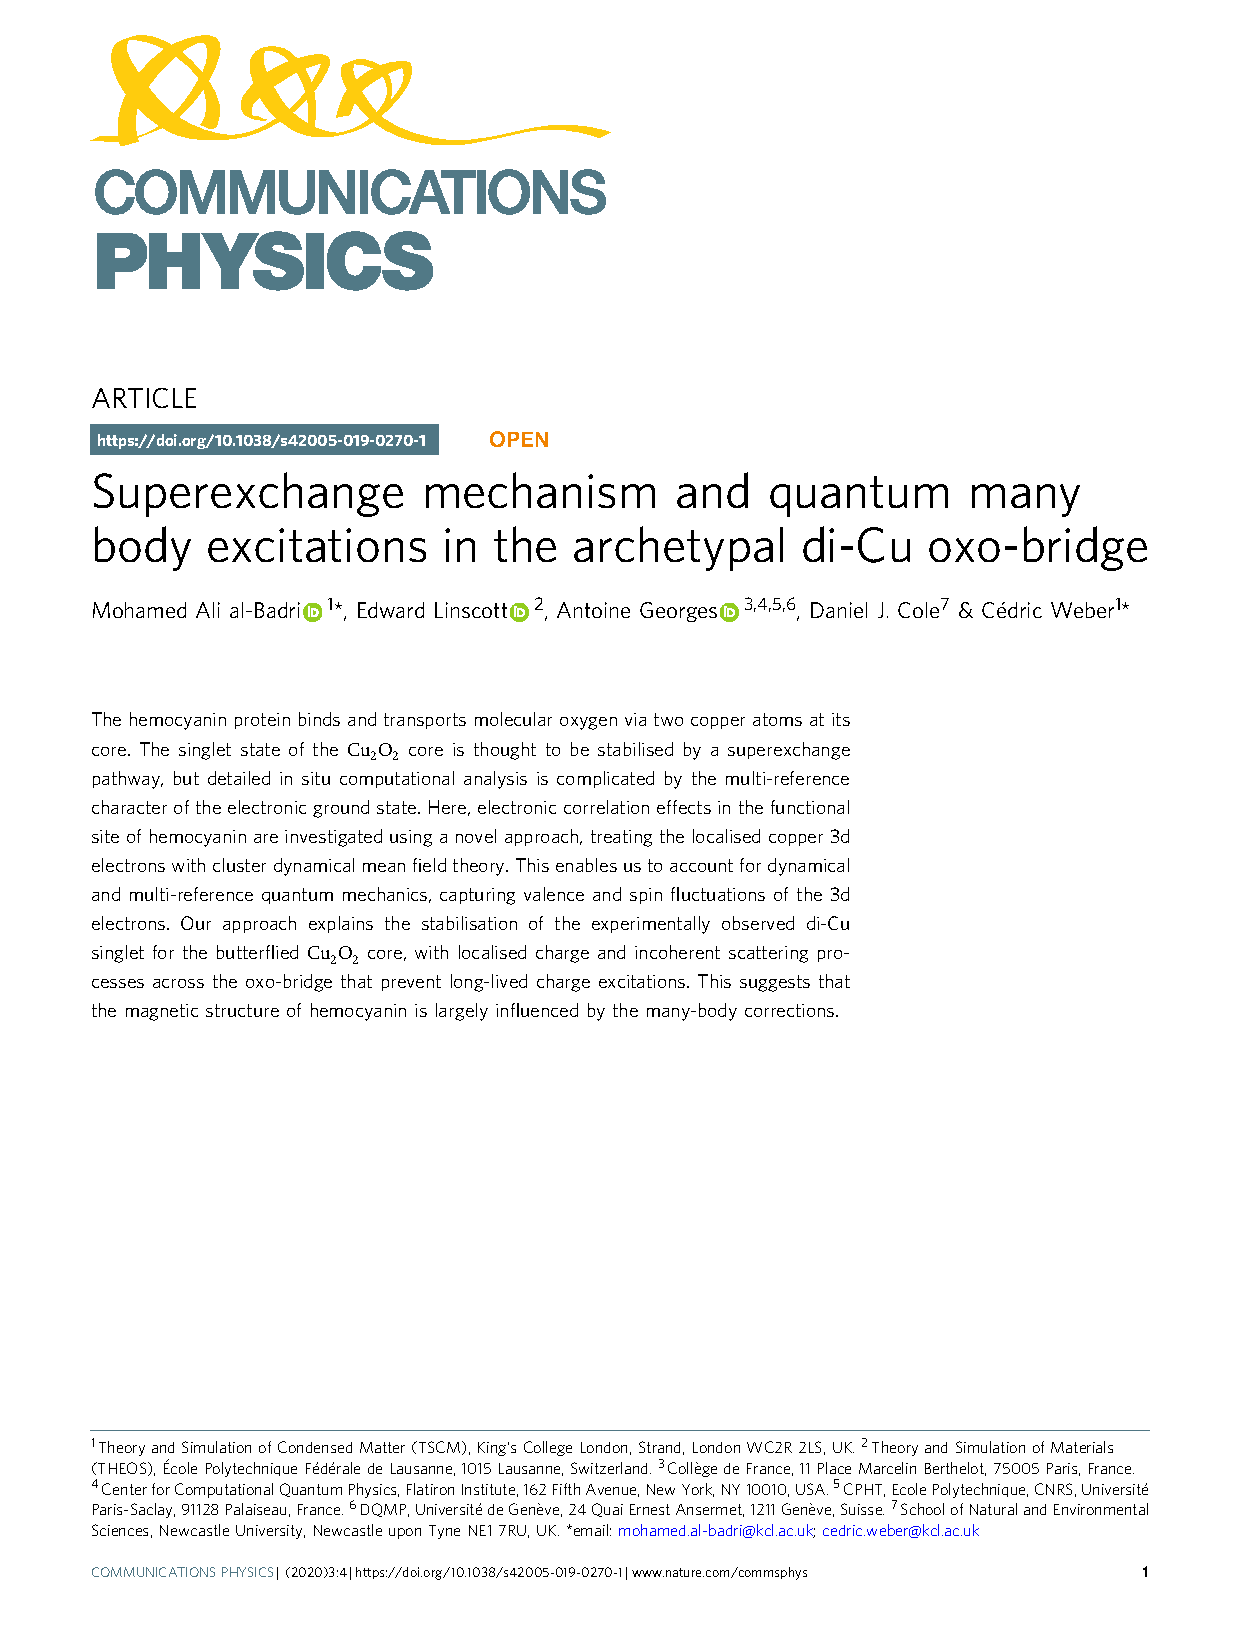
\includepdf[pages=-, offset=75 -75,addtotoc={
     2,section,1,Introduction,pp2,
     2,section,1,Results,pp2,
     2,subsection,2,The spin state of the Cu$_2$O$_2$ core,pp2,
     4,subsection,2,The superexchange mechanism,pp4,
     5,subsection,2,Optical transitions,pp5,
     5,section,1,Discussion,pp5,
     6,section,1,Methods,pp6,
     6,subsection,2,Geometry,pp6,
     6,subsection,2,Density Functional Theory,pp6,
     6,subsection,2,Dynamical Mean Field Theory,pp6},
     addtolist={
     3, figure,{\textbf{The oxyHc functional complex.} Structure showing the Cu$_2$O$_2$ correlated subsystem, which is treated using dynamical mean field theory, and the surrounding imidazole rings representing the protein environment. Hydrogen, carbon, nitrogen, oxygen and iron atoms are shown in white,green, blue, red, and orange respectively.},bb,
     3, figure, {\textbf{The superexchange model of Metz and Solomon.} The Cu$_2$O$_2$ core is depicted from side-on (a,c) and above (b,d). In the planar configuration (a,b), single-ligand orbitals bridge the two copper sites, and superexchange is possible. In a bent configuration (c,d), the copper \textit{d} orbitals overlap with different $\pi^{\ast}$ orbitals. As these two sets of orbitals are orthogonal, hopping between the blue and the red subspaces is not possible and the superexchange mechanism breaks down.},cc,
     4, figure, {\textbf{Decomposition of the reduced density matrix of the Cu$_2$ dimer in the different quantum sectors.} The colours correspond to the respective weights of the different contributions for each value of the Coulomb repulsion $U$ (if a colour occupies all the vertical axis, for example, it means that all eigenvectors of the density matrix are in that particular quantum sector). Note that the $d$ occupation is the sum of both Cu sites (e.g., $d^{20}$ means both Cu atoms are in the $d^{10}$ configuration).},dd,
     4,figure, { \textbf{Dynamical mean field self energy.} a) Imaginary part of the dynamical mean field local self energy $\Sigma(\omega)$ of the Cu-$3d$ empty orbital for Hubbard $U=2$\,eV, $6$\,eV, and $8$\,eV. At $U=8$\,eV, we obtain incoherent excitations at $\omega=0$\,eV. b) The imaginary local self energy at $\omega=0$ and c) the double occupancy of the partially-filled $3d$ orbitals $D$ as a function of $U$. Note that although the double occupancy is evolving smoothly with the Coulomb interaction $U$, $\Sigma(\omega=0)$ shows a sharp increase near $U=8$, associated with the stabilisation of a localised singlet },ee,
     5, figure, { \textbf{Molecular orbital isosurfaces.} The isosurface for the highest occupied molecular orbital (a, c) and lowest unoccupied molecular orbital (b, d) densities for $U = 8$\,eV, as viewed side-on (a, b) and above (c, d). Note that because these are extracted from the Green's function via the spectral density, the phase of the orbitals is inaccessible}, ff,
     5, figure, {\textbf{Theoretical optical absorption of the Cu$_2$O$_2$ core and imidazole rings obtained by dynamical mean field theory for values of the Coulomb repulsion $U=6$ to $10$\,eV.} For comparison, we show the experimental optical absorption in a wide range of wavelengths (infrared to UV). There are several smaller peaks in the experimental spectra that are not visible at this scale (indicated with arrows)}, gg}]{PDF_PAPERS/hemocyanin.pdf}

\includepdf[pages=-, offset=75 -75,addtotoc={
     1,section,1,Supplementary Figures,ppp1,
     4,section,1,Supplementary Notes, ppp4,
     4,subsection,2,Details of diamagnetism, ppp4,
     4,subsection,2,Von Neumann entropy, ppp4,
     5,subsection,2,Natural bond orbital analysis, ppp5,
     6,subsection,2,Atomic coordinates of the model system, ppp6,
     8,subsection,2,Convergence of the system-to-AIM mapping,ppp8,
     8,subsection,2,Local axes, ppp8},
     addtolist={
     1, figure,{The effective magnetic moment $M=\sqrt{\langle \mathbf{S}^2_1 \rangle/3}$  (normalised by saturation value) and the spin correlation $K=2\langle \mathbf{S}_1 \cdot \mathbf{S}_2 \rangle$ for varying values of the Hubbard $U$. For a pure two orbital singlet, $K=-1.5$. In our calculations, as the rest of the molecule hybridises with the Cu orbitals, the spin-correlation is re-normalised to half its saturation value for $U=6-8$\,eV.},aaa,
     1, figure,{The Von Neumann entropy $\Lambda$ of the reduced density matrix and its dependence on the on-site interaction $U$.},bbb,
     2, figure,{Isosurfaces of several natural bonding orbitals for $U = 8$\,eV. (a) Two Cu $3d$ orbitals are identified as half-filled by the NBO analysis. (b) The O\textsubscript{2} $\sigma^*$ anti-bond is empty, and does not hybridise with any Cu orbitals. (c) Instead, O $2p$ (blue) to Cu $4s$ (red) charge transfer is favourable.},ccc,
     2,figure,{(a) The local density of states for $U$ = 8\,eV and (b) the different total density of states of the Cu$_2$O$_2$ functional complex for a range of Hubbard $U$ values from DMFT.},ddd,
     3, figure,{The convergence of the distance $d$ as a function of the total number of sites (impurity and bath).}, eee,
     3, figure,{The local axes for the Cu $3d$ correlated subspaces, and the two half-filled NBOs for comparison.}, fff,
     4, table,{The DMFT $3d$ orbital occupations of Cu in our model of ligated hemocyanin for different Hubbard $U$ values, as calculated using NBO. Note that the orbital labels correspond to the local axes to each Cu atom. All eight other Cu $3d$ orbitals had occupancies $> 1.98$ for all values of $U$}, ggg}]{PDF_PAPERS/SI_hemocyanin.pdf}
%\includepdf[pages=-, offset=75 -75]{PDF_PAPERS/SI_hemocyanin.pdf}



